% !TeX spellcheck = en_US

\chapter{Foundations and Related Work}
\label{chap:ch2}
This chapter outlines other work relevant to this thesis.
First, the foundations are described in \cref{sec:ch2:s1}.
Then \cref{sec:ch2:s2} introduces and discusses other work in this research area, 
discovered using the process described in \cref{ssec:ch2:ss2.1}.

\section{Foundations}
\label{sec:ch2:s1}
This section describes the foundations this work is based on and which may be useful for understanding this thesis.
First, in \cref{ssec:ch2:ss1.0} the query language \gls{graphql} is  introduced.
After that, \cref{ssec:ch2:ss1.1} covers the idea of software issues and issue management systems in general.
Then, in \cref{ssec:ch2:ss1.2}, a concept for issue management in environments where multiple software components, 
which are developed by independent teams, is described.
\Cref{ssec:ch2:ss1.3} introduces the concept of \glspl{IDE} and how they can be extended 
with a focus on \gls{Eclipse} as the prototype developed for this thesis is an \gls{Eclipse} plugin.
Finally, \cref{ssec:ch2:ss1.4} covers two frameworks used in the implementation of that plugin.

\subsection{GraphQL}
\label{ssec:ch2:ss1.0}
\gls{graphql} is a query language developed by Facebook, where the client needs to specify the parts of data to return \cite{grpahql2018}.
Furthermore, changed data cannot just be sent to the server to be updated, but the changes must be recorded and split into so-called mutations,
which can then be sent to the server.

\subsection{Software Issues and \acrlongpl{IMS}}
\label{ssec:ch2:ss1.1}
Software issues are a way to communicate a need for action in the software engineering process.
Traditionally, a distinction was made between a bug, which needs to be debugged or fixed, a task someone needs to do, 
and an enhancement being requested.
Issues can represent any of these things as well as anything a developer needs them to represent \cite{Atlassian2020Issue,Github2020Issues}.

\glspl{IMS}, also called Issue Tracking Systems, are programs, which maintain these issues 
and ``help organizations manage issue reporting, assignment, tracking, resolution, and archiving'' \cite{bertram2010communication}.
Other common names include bug tracker, defect tracker, and ticket system.
They can bring various benefits like improved software quality, request accountability, and 
an increase in productivity \cite{janak2009issue}. 

Software issues typically consist at least of a title, a detailed description or body text, and a state, 
which typically has at least the possible values open and closed.
Additionally, each \gls{IMS} supports various additional fields like the type (bug, enhancement, task, etc.), 
labels to further classify the issue, relevant parts of the source code, the creation date, a due date, the issue creator, the developer(s) assigned to work on it, or many more.
However, the amount of supported fields varies greatly between different programs.

Common \glspl{IMS} include Atlassian's Jira\footnote{\url{https://www.atlassian.com/software/jira}}, 
Bugzilla\footnote{\url{https://www.bugzilla.org/}} 
as well as the issue management support integrated into Redmine\footnote{\url{https://www.redmine.org/}}, 
GitHub\footnote{\url{https://github.com/}} and 
GitLab\footnote{\url{https://gitlab.com/}}.
Most provide various features in addition to just storing these issues. 
Those features include linking related issues, grouping issues into so-called Milestones, organizing issues on project boards, similar to the Kanban Boards described by Thomas Epping \cite{epping2011kanban}, advanced time tracking, and more.
An in-depth comparison of a few well known \glspl{IMS} is provided by Jan{\'a}k, Ji{\v{r}}{\'\i} \cite{janak2009issue}. 

\subsection{Issue Management in Multi-Team, Multi-Component Environments (Gropius)}
\label{ssec:ch2:ss1.2}
Managing documentation and issues for multi-project, multi-team scenarios efficiently is a major problem for the software development process  \cite{mahmood2015identifying}. This assertion is supported by some posts in forums of Jira and Redmine asking for solutions to this problem\footnote{\url{https://www.redmine.org/boards/1/topics/21939}}\footnote{\url{https://community.atlassian.com/t5/Jira-questions/How-do-others-work-with-issues-affecting-multiple-projects/qaq-p/399950}}\footnote{\url{https://community.atlassian.com/t5/Jira-Software-questions/Share-one-issue-quot-ticket-quot-across-multiple-projects-and/qaq-p/407534}}. Another strong argument supporting it are the results of an expert survey conducted by Sandro Speth \cite{Speth2019}, which indicate that industry experts also see this as a problem.

One possible approach to deal with this problem is introduced in \cite{Speth2019}.
The proposed solution are so-called multi-project coding issues. These are issues concerning multiple projects and, therefore, are stored in the issue management system of each relevant project. 
Additionally, traceability links between multiple issues and artifacts are proposed. 
For example, one issue about a crash could link to another issue describing the Exception causing the crash, which in turn links to the piece of code causing it and the part of the architecture specification involved.
As a concrete syntax, a graphical notation for these issues and links is introduced and implemented in a prototype framework. The frontend of this framework is a web-based application with an architecture graph at its core.
This graph is used to view and edit the system architecture and issues displayed with the introduced notation. 

Speth et al. \cite{speth2020gropius} further refine this concept and introduces a tool named \gls{Gropius}, which is  based on the prototype mentioned above.
Among other things, the paper presents the architecture of the \gls{Gropius} system. 
One relevant fact for this thesis is, that the \gls{Gropius} back-end provides a \gls{graphql} \gls{API} for the front-end,
which can also be used by the tool of this thesis.
The \gls{Gropius} system does not store just store the issues in its own database, but works with one or more traditional \glspl{IMS} to retrieve and store the issues.
Therefore, the system can be used by some developers without causing problems for other colleagues not using it.

\begin{figure}[!h]
	\centering
	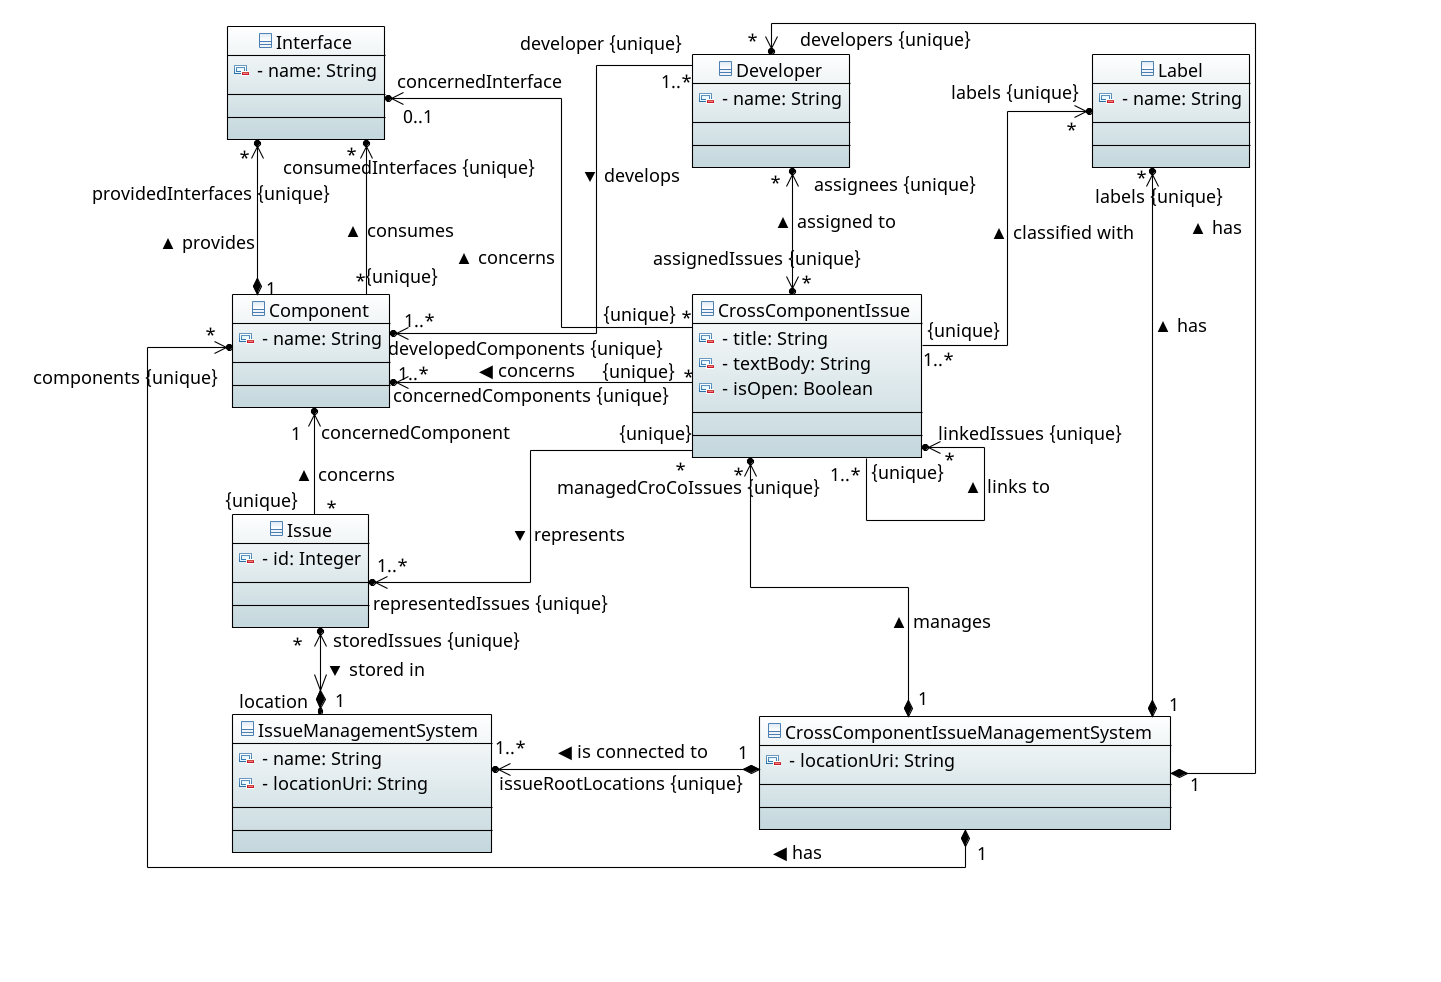
\includegraphics[width=\textwidth]{graphics/domainMetaModel.png}
	\caption{Domain meta Model of the \gls{Gropius} system \\ \footnotesize{The same figure can be found enlarged in \cref{chap:appendix:design_docs}}}
	\label{fig:c2:domain_meta_model}
\end{figure}

It also introduces a domain meta model for the \gls{Gropius} system, as depicted in \cref{fig:c2:domain_meta_model} \cite{speth2020gropius}.
At the center you can see the Cross-Component-Issue, which represents multiple normal issues.
These Cross-Component-Issues are stored in the Cross-Component-Issue-Management-System, for example an instance of the \gls{Gropius} system.
That is connected to multiple traditional \glspl{IMS}, which hold the normal issues.
In addition to some simple attributes like the title, text body, and the flag for whether the issue is open, a Cross-Component-Issue also has references to the assigned developers, its labels, and the components or interfaces it occurs in.

\subsection{Extending \acrlongpl{IDE}}
\label{ssec:ch2:ss1.3}
An \gls{IDE} is a software tool for programming, which typically has a rich text editor at its core 
and contains various other tools for use during software development.
The concept of a dedicated software \gls{IDE} can be traced back to the Maestro I system, first called ``Programm-Entwicklungs-Terminal-System'' (program development terminal system), short PET, developed by Softlab Munich reported about in \cite{Computerwoche1975Ide}.
Well known \glspl{IDE} today include Visual Studio\footnote{\url{https://visualstudio.microsoft.com}}, \gls{Eclipse}\footnote{\url{https://www.eclipse.org/ide/}}, NetBeans\footnote{\url{https://netbeans.org}}, IntelliJ IDEA\footnote{\url{https://www.jetbrains.com/idea/}}, and Visual Studio Code\footnote{\url{https://code.visualstudio.com/}} .

Various \glspl{IDE} follow the general trend to allow extending a piece of software with the help of plugins \cite{chang2008issues}.
This enables developers to add custom features or integrated support for previously unsupported external tools.
The concept of integrating many tools into one environment was already investigated in 1990 by Anthony I. Wasserman \cite{wasserman1990tool}.

One of those is \gls{Eclipse}, originally being developed by IBM using \gls{java} as proprietary software.
It was open-sourced in 2001 and is maintained by the Eclipse Foundation\footnote{\url{https://www.eclipse.org/org}}
today \cite{burnette2005eclipse}.
Originally, it was intended as a \gls{java} \gls{IDE} but with the help of plugins support for many programming languages can be added today.
According to various online rankings\footnote{\url{https://pypl.github.io/IDE.html}}\footnote{\url{https://www.positronx.io/top-10-best-ide-for-software-development/}},
\gls{Eclipse} is one of the most popular \glspl{IDE} at the time of writing.

Eclipse is designed to be extended by plugins. This is regularly done by the industry as well as by researchers 
because it is a simple way to create a large and powerful tool containing custom features 
without requiring the effort to build a complete tool from scratch. 
Recent papers using Eclipse as the base of their tool are for example \cite{segura2019extremo} or \cite{hajji2019onto2db}. 
The process of creating an Eclipse plugin is explained in great detail by Clayberg et al. \cite{clayberg2006eclipse}.

\subsection{The \acrlong{EMF} and \gls{Parsley} }
\label{ssec:ch2:ss1.4}
One alternative for manually implementing every part of a program is \gls{MDSD}.
With this approach, most of the software is modeled using some modeling language or tool and then generated \cite{volter2013model}. 

The \gls{EMF} is a framework for \gls{MDSD} optimized for use with \gls{Eclipse}.
At its core is the Ecore meta-model, with which models are represented \cite{steinberg2008emf}.
Such an Ecore model can for example be obtained by converting an existing \gls{UML} model.
From that, the complete source code for the data structure represented by the model can be generated.
The generation of other components such as editors is also supported but not used in this thesis.

\Gls{Parsley} is a framework on top of \gls{EMF} for creating \glspl{UI}.
It allows developers to build an \gls{Eclipse} \gls{UI} based on a data model generated by \gls{EMF} with very little setup \cite{bettini2014developing}.
Developers can use existing \gls{UI} elements provided by \gls{Parsley} and customize them to their needs using injected aspects  \cite{bettini2014developing}.
One core feature is the integrated \gls{DSL} allowing developers to specify the desired \gls{UI} in a simple language \cite{bettini2014developing}.

\section{Related Work}
\label{sec:ch2:s2}
First, the methodology used for finding the related work is presented in \cref{ssec:ch2:ss2.1}.
Then the related academic work found is introduced in \cref{ssec:ch2:ss2.2}.
Finally, \cref{ssec:ch2:ss2.3} covers existing issue management plugins for eclipse.

\subsection{Literature Research Methodology} 
\label{ssec:ch2:ss2.1}
The following procedure was used for finding related work:
First, an initial search was performed using the search terms below and Google Scholar\footnote{\url{https://scholar.google.com}} as the search engine.
Of each query, the top ten results were taken and examined.
First, results were rejected based on their title and the short excerpt Google Scholar includes in the search results page, 
then based on the abstract.
All remaining results were examined in depth to check whether they can be considered related work.
Finally, the same process was repeated with all references to English papers of any work found, 
which was classified as related work until no more such papers were identified (Snowballing).

The build the search terms all possible combinations of the following two parts were used.
For part number one the following terms were used:
\begin{itemize}
	\item IDE
	\item Integrated development environment
	\item Eclipse
\end{itemize}

For the second part these terms were used:

\begin{itemize}
	\item issue management
	\item issues
	\item issue trackers
	\item bug tracker
	\item defect tracker
\end{itemize}

This makes a total of 15 search terms resulting in 150 results, only considering the first ten results.
After sorting by title and excerpt a total of nine unique results remained, three after reading the abstract, and two after further analysis.
Of these two papers, the first had 12 references, of which all were rejected based on the title and the second had 18 references in the relevant section, of which also none could be identified as relevant for this work.

Additionally, the eclipse marketplace\footnote{\url{https://marketplace.eclipse.org}} was searched using the terms ``issue management'', ``defect'', and ``defects''. 
All results were searched for appropriate plugins.
The term ``bug'' could not be used to search the marketplace, because over 200 plugins were found and on the first few pages, most results were not relevant.

\subsection{\gls{IDE} Support for Issue Management in Academia} 
\label{ssec:ch2:ss2.2}
Only two papers about the integration of issue management into an \gls{IDE} could be found.
This indicates, that not a lot of research has been done in this area.

The first of the two papers is \cite{iqbal2009integrating},
which includes a short section on integrating their custom framework called ``Linked Data Driven Software Development (LD2SD)'' 
into the \gls{Eclipse} \gls{IDE}.
LD2SD allows searching in various software development artifacts like documentation or issues.
However, the only integration into \gls{Eclipse} presented in the work is the ability to perform a query based on 
parts of the source code (like a class or method) within \gls{Eclipse} and the result would be shown in the integrated web browser provided by \gls{Eclipse} \cite{iqbal2009integrating}.
They show that such a query can be started by a custom element in the context menu of \gls{java} class files in the \gls{Eclipse} package explorer.

Similarly to theirs, the goal of this thesis is to integrate an existing framework into the \gls{Eclipse} \gls{IDE} with the help of a plugin.
However, in contrast to them, this work only focuses on issues but aims to provide much more extensive support to work with those, like adding custom \gls{UI} elements to view and edit them.

The second related work found is \cite{janak2009issue}.
It first gives an overview of existing issue management plugins for \glspl{IDE} and then describes the process for developing an ``Atlassian NetBeans Connector''.

In the overview, the author differentiates between two kinds of plugins realizing the integration of issue management into \glspl{IDE}.
According to the author the first kind is a ``Universal plug-in with bridge for connecting the issue tracking system'',
which allows the easy integration of multiple \glspl{IMS} by providing an interface, which can be implemented by so-called bridges, 
each attaching a single \gls{IMS} to the universal plugin.
The core of this universal plugin is then responsible to work with the \gls{IDE} to show the retrieved issues to the user.
The author states, that this kind of issue management plugin generally does not support advanced features of the individual \glspl{IMS}.
The second kind is the ``Single issue tracking system plug-in'' \cite{janak2009issue}, which typically supports most features of a single \gls{IMS}.

For the first kind, he describes Mylyn for \gls{Eclipse}, which is discussed in detail in \cref{ssec:ch2:ss2.3} as well as Cube°n for Netbeans.
Cube°n\footnote{\url{https://code.google.com/archive/p/cubeon/}} is a task-focused \gls{UI} for NetBeans similar to Mylyn, which was originally started at Google's ``Summer of Code`` in 2008 \cite{janak2009issue}.
It has since been renamed to Task Focused NetBeans\footnote{\url{http://wiki.netbeans.org/TaskFocusedNetBeans}} and is being maintained by the NetBeans team and community.

For the second kind the paper introduces two plugins for the \gls{IMS} CodeBeamer ALM by Intland Software\footnote{\url{https://codebeamer.com/}}, one for \gls{Eclipse} and one for NetBeans, as well as the ``Atlassian IDE Connector'' for IntelliJ IDEA and \gls{Eclipse}.
According to the author, the CodeBeamer ALM is a good issue management plugin supporting all CodeBeamer ALM features with a simple and intuitive \gls{UI}.
Both Atlassian Connectors allow the use of various Atlassian products, including Jira, in the \gls{IDE} \cite{janak2009issue}.
The author states that the connector for IntelliJ IDEA is a lot more advanced than the one for \gls{Eclipse}, which is based on Mylyn.
The Atlassian Connector for \gls{Eclipse} is also covered in \cref{ssec:ch2:ss2.3}.

Then the work describes the concept, design, and implementation of a new Atlassian connector for NetBeans, with the Jira connector being the primary goal.
According to the author, it is primarily inspired by the above mentioned Atlassian IntelliJ IDEA connector.
The created Jira integration allows users to view a filtered list of issues, a specific issue as well as their comments, create a new issue or comment, log work on an issue, view stack traces from an issue, and click through to the relevant source file, assign an issue to someone and perform workflow actions (similar to changing the state) on a selected issue.

That work provides a much more advanced integration than the previous one, with a similar amount of features to the one presented in this thesis.
On the other hand, the plugin presented in it only works with the Jira \gls{IMS} in contrast to the one of this thesis which integrates into the \gls{Gropius} framework, which theoretically can work with any \gls{IMS}.
Additionally, theirs is for NetBeans, while ours is for \gls{Eclipse}.

However, the most important difference between this thesis and the two covered related works
is the fact that, in contrast to the other two, the tool presented in this thesis has support for the features of \gls{Gropius},
which are intended to help with the issue management in component-based, multi-team environments.


\subsection{Issue Management Plugins for Eclipse}
\label{ssec:ch2:ss2.3}
Compared to academia, the industry has put a little more work into this area.
There exist a few issue management plugins for various \glspl{IDE} \cite{janak2009issue}, 
but in this section, the focus is on issue management plugins for \gls{Eclipse}.
In total five issue management plugins for \gls{Eclipse} could be found.
Four, which are specific to one \gls{IMS} and one universal plugin using bridges to connect to many \glspl{IMS}.

The first is ``Teamscale Integration for Eclipse''\footnote{\url{https://marketplace.eclipse.org/content/teamscale-integration-eclipse}}, 
which allows users to browse the defects found by a Teamscale software‐quality analysis server.
This server is not a typical \gls{IMS}, but rather a software analyzing the source code for potential issues.

The second is called ``CollabNet Desktop''\footnote{\url{https://marketplace.eclipse.org/content/collabnet-desktop-eclipse-edition}} and 
integrates with the application lifecycle management platforms of CollabNet, which include issue management and can therefore be called \gls{IMS} in the context of this thesis.

The next is ``JiraBuddy - Eclipse Plugin for JIRA''\footnote{\url{https://marketplace.eclipse.org/content/jirabuddy-eclipse-plugin-jira}}
is a plugin adding various enhancements when working with Atlassian Jira and \gls{Eclipse}, but does not provide the capability to create or update 
issues from within \gls{Eclipse}. According to their website\footnote{\url{http://home.jirabuddy.com/}}, the only feature is to display the issue when hovering over the corresponding issue identifier in the \gls{Eclipse} editor.

The last plugin of this kind is ``Atlassian Connector for Eclipse''\footnote{\url{https://marketplace.eclipse.org/content/atlassian-connector-eclipse}}.
It not only provides integration into Atlassian Jira, which is relevant for this thesis, but also other Atlassian products like the Bamboo continues integration and deployment server.
It is actually built on top of Mylyn, which is explained below.

All of the above only work with one specific \gls{IMS}, whereas the tool proposed by this thesis can work with any \gls{IMS} supported by \gls{Gropius}.
Additionally, the last two of them are not maintained anymore and, therefore, have no support for current \gls{Eclipse} versions. 

The fifth and most important plugin is Mylyn\footnote{\url{https://marketplace.eclipse.org/content/mylyn}} together with its many connectors for various \glspl{IMS}.
It is one of the oldest issue management plugins for any \gls{IDE} \cite{janak2009issue}.
At its core is a list of tasks, which can contain local tasks stored on the computer and tasks provided by one of the many connectors.
One important concept is the task-focused interface, which means Mylyn tries to highlight the parts of the \gls{Eclipse} \gls{UI} relevant to the current task and makes the less relevant parts less prominent.
That mainly applies to the \gls{Eclipse} package explorer, where different resources and files will be drawn with different shades of gray based on their relevance for the current task.
Data about the relevancy of parts for the current task is extracted from the user's behavior.
But in contrast to the solution provided in this thesis, Mylyn can only associate issues, or tasks as they are called in Mylyn, to resources as specific as source code files and not to lines within them.

Similar to the academic work, all these plugins lack support for all or some features necessary in component-based, multi-team environments,
like one issue being saved in multiple different \glspl{IMS} of multiple teams or the ability to quickly navigate between related issues.

